\documentclass[conference]{IEEEtran}
\IEEEoverridecommandlockouts
% The preceding line is only needed to identify funding in the first footnote. If that is unneeded, please comment it out.
\usepackage{cite}
\usepackage{amsmath,amssymb,amsfonts}
\usepackage{algorithmic}
\usepackage{graphicx}
\usepackage{textcomp}
\usepackage{xcolor}
\usepackage{array}
\def\BibTeX{{\rm B\kern-.05em{\sc i\kern-.025em b}\kern-.08em
    T\kern-.1667em\lower.7ex\hbox{E}\kern-.125emX}}
\begin{document}

\title{Online Bandit Learning-Based Multi-Mode State-Retentive Power Gating for HPC Systems\\
\thanks{This work was supported by the Center for Heterogeneous Integration of Micro Electronic Systems (CHIMES), one of seven centers in Joint University Microelectronics Program (JUMP) 2.0, a Semiconductor Research Corporation (SRC) program sponsored by the Defense Advance Research Project Agency (DARPA).}
}

\author{
\begin{minipage}[t]{\linewidth}
    \centering
    Salma Abdelzaher, Mohamed Gharib, Amit Ranjan Trivedi and Inna Partin-Vaisband\\
    University of Illinois Chicago\\
    Chicago, IL, USA \\
    sabdel29@uic.edu, mghari5@uic.edu, amitrt@uic.edu, vaisband@uic.edu
\end{minipage}
\hfill
}

% \and
% \IEEEauthorblockN{5\textsuperscript{th} Given Name Surname}
% \IEEEauthorblockA{\textit{dept. name of organization (of Aff.)} \\
% \textit{name of organization (of Aff.)}\\
% City, Country \\
% email address or ORCID}
% \and
% \IEEEauthorblockN{6\textsuperscript{th} Given Name Surname}
% \IEEEauthorblockA{\textit{dept. name of organization (of Aff.)} \\
% \textit{name of organization (of Aff.)}\\
% City, Country \\
% email address or ORCID}

\maketitle

\begin{abstract}
In deep submicron nodes, leakage power is a critical concern, especially in high-performance computing (HPC) and advanced 2.5D/3D integration, where traditional power gating techniques struggle with adaptability and responsivness. This paper proposes a novel multi-mode, state-retentive power gating architecture integrated with an online bandit learning algorithm for real-time sleep mode selection under workload-driven idle patterns. Unlike heuristic or pre-learned strategies, the proposed multi-armed bandit (MAB) controller adapts on-the-fly to stochastic idle distributions caused by dynamic memory access patterns and decentralized dynamic voltage and frequency scaling (DVFS) operations. Implemented in 65 nm CMOS technology node and validated in Cadence Virtuoso on SRAM logic, the design demonstrates leakage reductions of 92.5\%–98\% across modes. The adaptive MAB controller further achieves up to 71.7\% energy savings compared to state-of-the-art (SOTA) approaches. The approach is robust across process, voltage, and temperature (PVT) corners and provides a lightweight, scalable solution tailored for idle-prone HPC workloads.


\end{abstract}

\begin{IEEEkeywords}
High performance computing (HPC), leakage, power consumption, power gating, bandit algorithm, multiple sleep modes, reinforcement learning.
\end{IEEEkeywords}

\section{Introduction}

Leakage power remains a significant contributor to total power dissipation in heterogeneous (2.5D) and three-dimensional (3D) integrated circuits (ICs) designed at sub-10nm technology nodes—platforms considered among the most promising for enabling high-performance computing (HPC) and AI applications \cite{ECTCSal,ECTC, Inna_book}. Power gating is widely used to mitigate static power by disconnecting idle blocks from the supply, but its efficiency depends heavily on accurately predicting idle durations and minimizing transition overheads. While self-adaptive gating techniques with embedded learner circuits have been proposed \cite{6807809}, their effectiveness is limited by the latency of the observation-and-response cycle (i.e., the time required to gather enough activity information before deciding to power gate the system). This delay reduces their practicality under short or highly variable idle phases.

Multi-mode power gating offers a more granular approach by enabling hardware blocks to enter multiple low-power states, such as shallow and deep sleep, depending on the expected idle time \cite{1613208}. Shallow modes allow rapid wake-up with modest leakage savings, while deep modes provide greater savings at the cost of longer recovery and potential state loss. State-retentive designs partially address this but often support only a single mode \cite{patent}. FD-SOI solutions with body biasing are another alternative, but they require process-specific modifications and additional integration effort \cite{7593216}.
\begin{figure}[t]
    \centering
    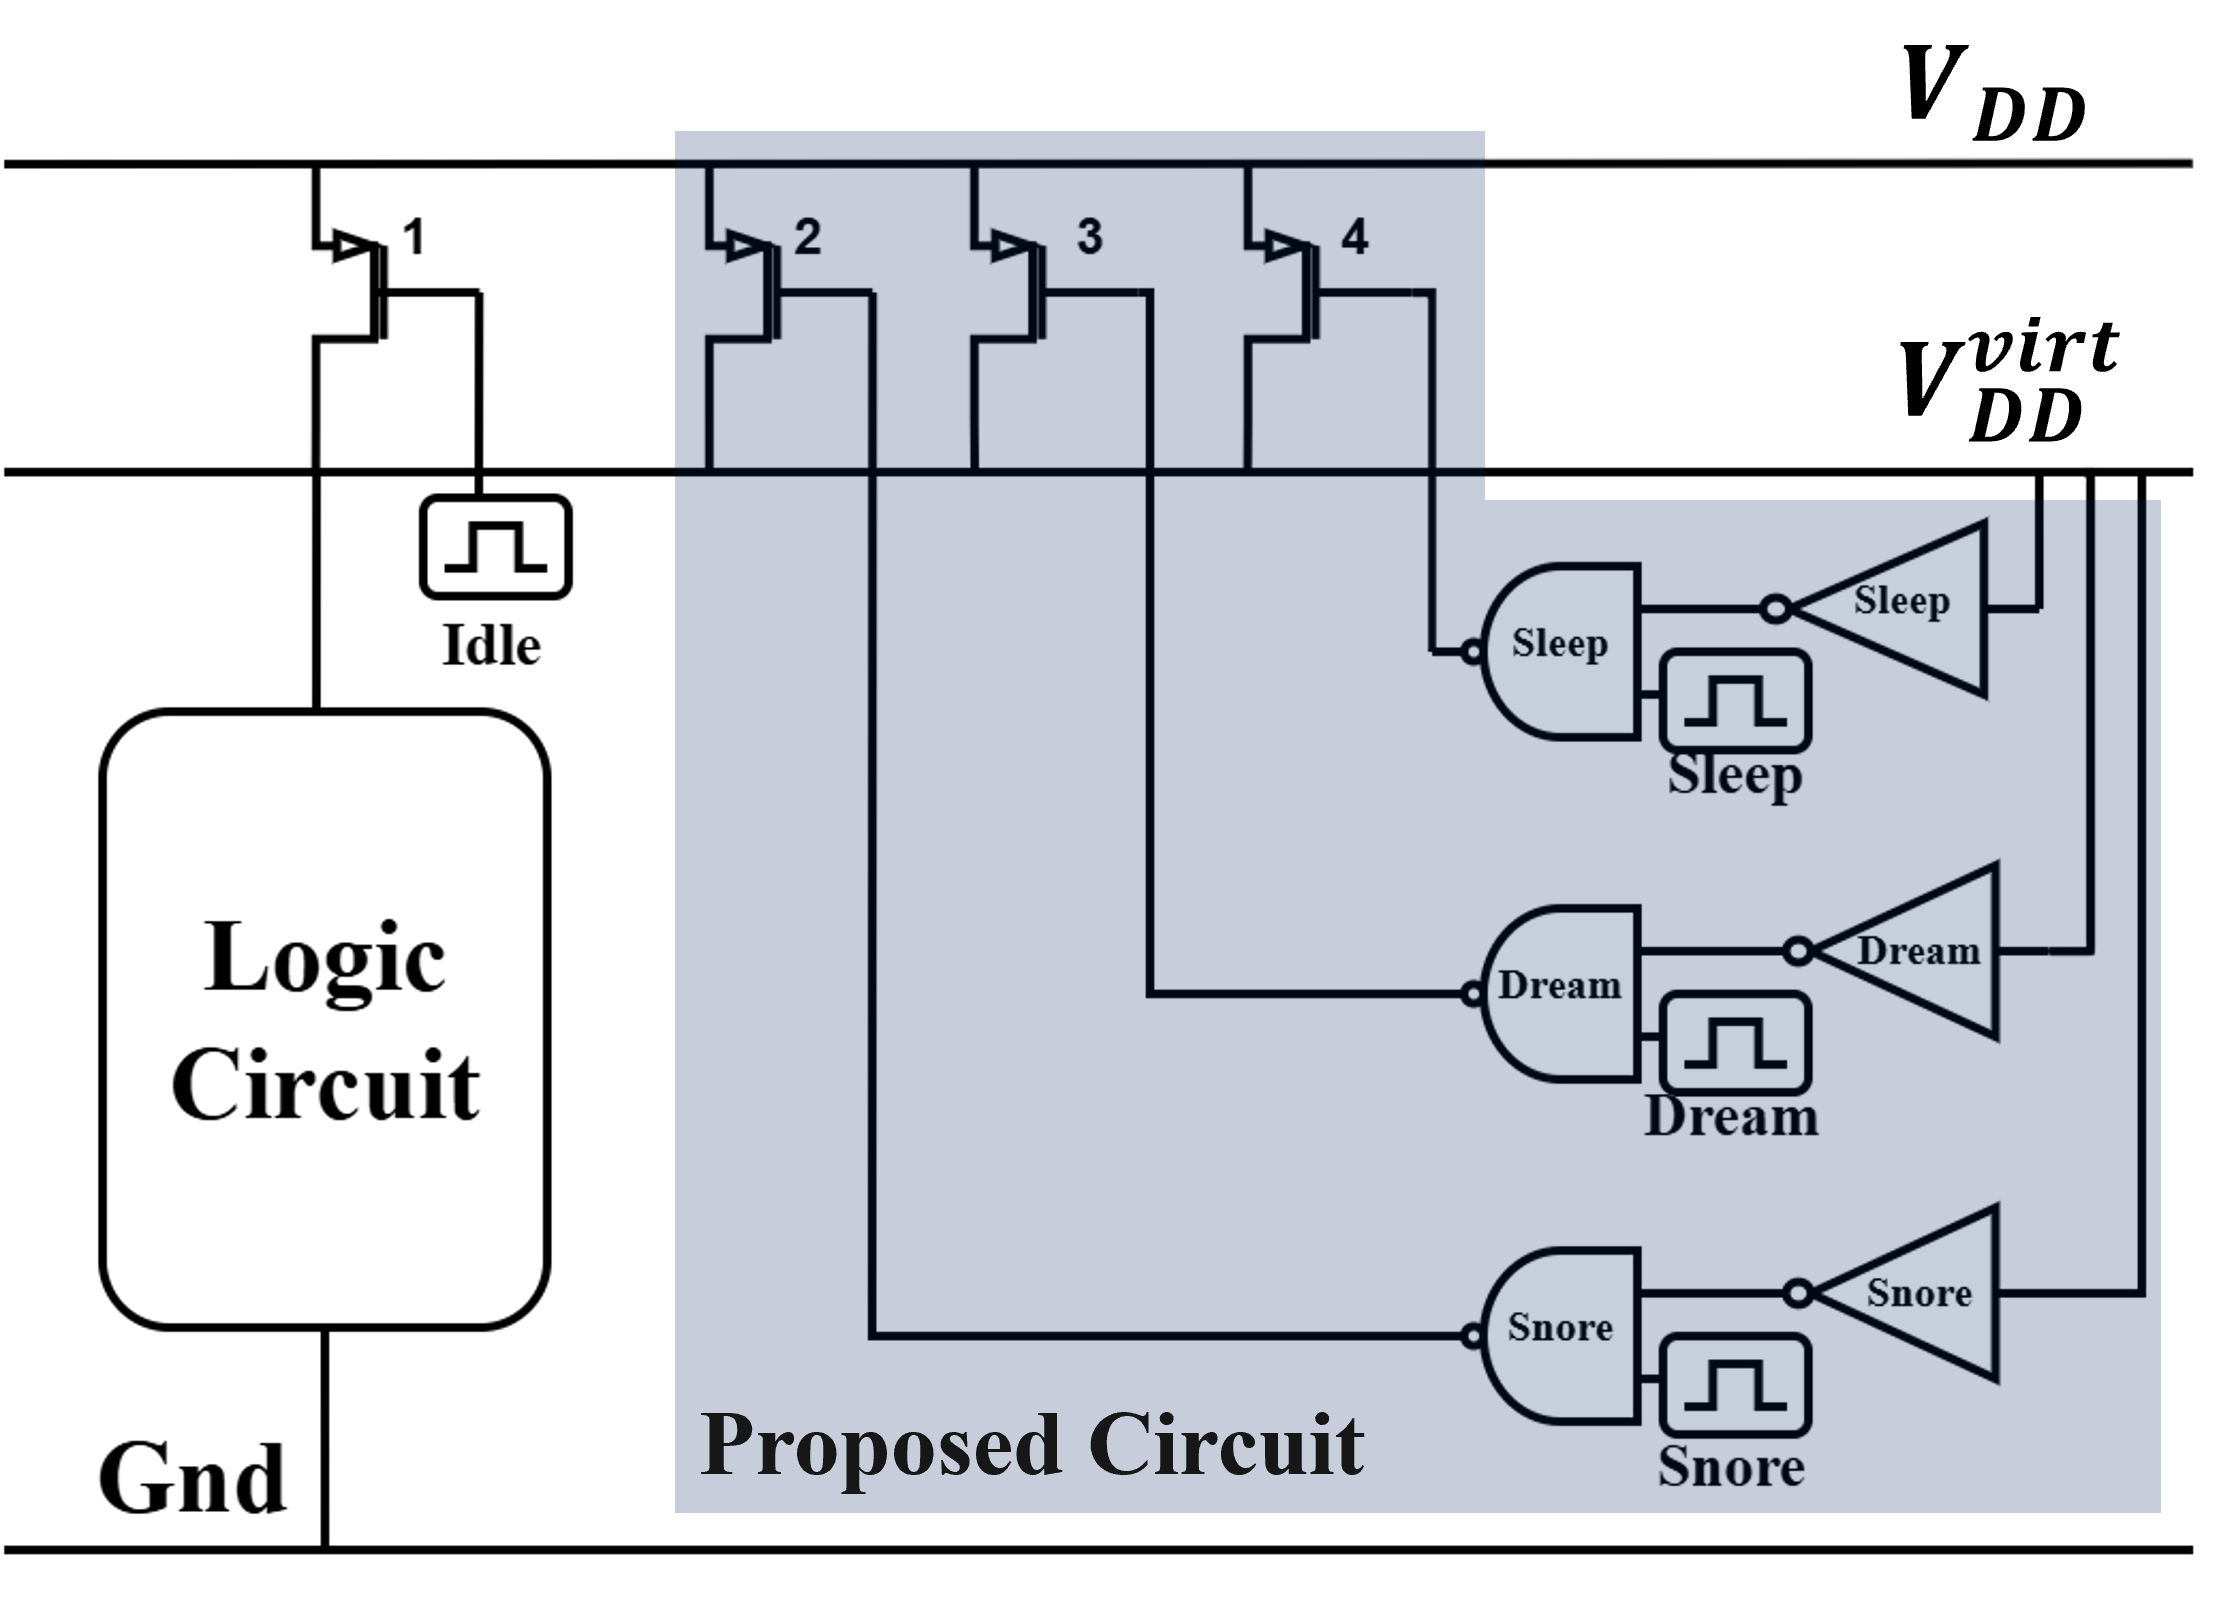
\includegraphics[width=0.45\textwidth]{PG_Ckt_newww.png}
    \caption{Proposed state-retentive multi-sleep mode power gating circuit. The Sleep, Dream, and Snore inverters differ by their switching threshold voltage, $V_{sw_{th}}^{Sleep} > V_{sw_{th}}^{Dream} > V_{sw_{th}}^{Snore}$.}
    \vspace{-10pt}
    \label{proposed_PG_Ckt}
\end{figure}

To address these limitations, we propose a compact, state-retentive, multi-mode power gating architecture in 65nm CMOS, validated on SRAM logic using Cadence Virtuoso. The design achieves substantial leakage reduction across a wide range of idle durations, without incurring area or process overhead. To handle the unpredictability and stochastic nature of real-world idle patterns, we introduce a lightweight online machine learning controller based on MAB algorithms. Unlike traditional ML approaches that rely on offline training or large inference pipelines, our MAB-based method operates online with negligible computational cost and learns dynamically by continuously observing system activity and selecting the most energy-efficient sleep mode on the fly.

This dynamic mode selection is critical for responsiveness and adaptability—fixed heuristics or pre-characterized strategies are insufficient under HPC workloads, where idle phases vary significantly due to memory accesses and autonomous DVFS decisions across cores. By minimizing both leakage and wake-up cost in real time, the proposed controller ensures consistent energy efficiency under varying process, voltage, and temperature (PVT) conditions. The resulting solution is ideally suited for frequently idle and energy-hungry HPC systems, where both performance and power budgets are tightly constrained.



%Leakage power remains a significant contributor to total power dissipation in heterogeneous (2.5D) and three-dimensional (3D) integrated circuits (ICs) designed at sub-10 nm technology nodes---platforms considered among the most promising for enabling high-performance computing (HPC) and AI applications \cite{ECTCSal,ECTC}. Power gating is widely employed to mitigate static power by disconnecting idle blocks from the supply. However, its efficiency depends on accurately predicting idle durations and minimizing transition overheads. Self-adaptive gating techniques with learner circuits have been proposed, yet their learning latency limits effectiveness during short or unpredictable idle phases \cite{6807809}.

%Multi-mode power gating offers a more flexible solution, enabling circuits to enter shallow or deep sleep states based on idle patterns \cite{1613208}. Shallow modes offer quick wake-up and modest leakage savings, while deep modes provide higher savings at the cost of longer recovery times and state loss. FD-SOI solutions with body biasing provide another alternative but incur additional integration and fabrication complexity \cite{7593216}.

%A compact state-retentive multi-mode power gating architecture is proposed in this paper. The architecture is designed in 65 nm CMOS and validated using SRAM logic in Cadence Virtuoso. The system achieves substantial leakage reduction with minimal area overhead and no additional process complexity. Robustness to global variations is ensured through co-localization with the gated logic. To further enhance responsiveness, the optimal sleep mode is dynamically selected with a lightweight bandit-based controller based on idle behavior and energy-latency trade-offs. The proposed solution is well-suited for idle-prone energy-constrained HPC systems.


\section{Proposed Power Gating Circuit and Operation}
\label{proposed Circuit and operation}


\begin{figure}[t]
    \centering
    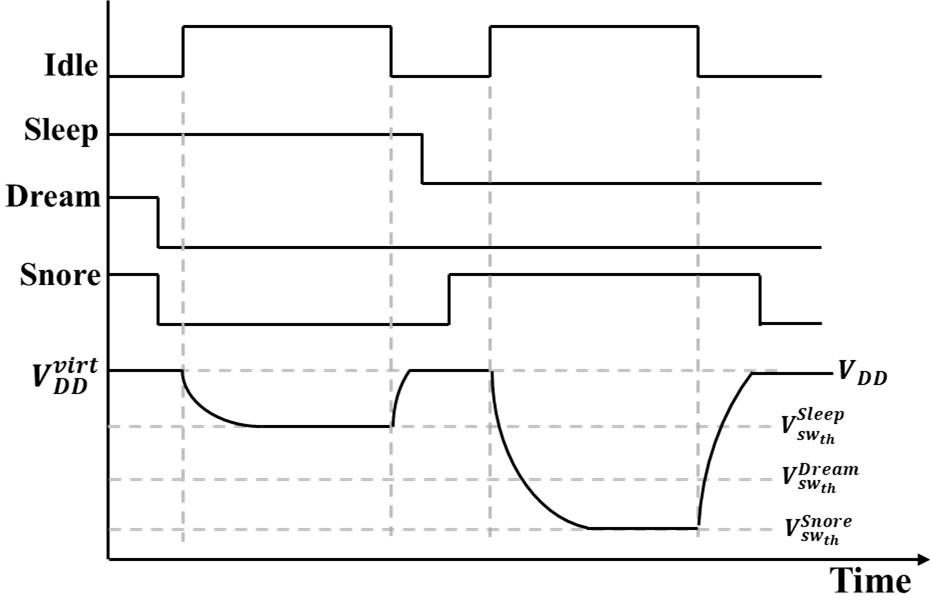
\includegraphics[width=0.4\textwidth]{timing_2.png}
    \caption{Timing diagram illustrating the dynamic regulation of $V_{DD}^{virt}$ across sleep, dream, and snore modes.}
    \vspace{-10pt}
    \label{timing}
\end{figure}

Disconnecting the logic circuit's virtual supply voltage ($V_{DD}^{virt}$) from the main supply ($V_{DD}$), limits all internal node voltages---including the gate and drain voltages---to a maximum of $V_{DD}^{virt}$. According to the subthreshold leakage current model~\cite{wang2006subthreshold},

\begin{equation}
    I_{sub} = I_{D0} \times e^{\frac{V_G}{mV_T}} \times (e^{\frac{-V_S}{V_T}} - e^{\frac{-V_D}{V_T}}),
\end{equation}
where, $I_{D0}$ is a technology dependent characteristic current, $V_T$ is the thermal voltage, and $V_G$, $V_S$ and $V_D$ are the gate, source and drain voltages, respectively. Reducing these voltages exponentially decreases the subthreshold leakage current, thereby lowering leakage power.

The proposed circuit regulates the $V_{DD}^{virt}$ across three distinct power gating modes Sleep, Dream, and Snore, offering a trade-off between leakage power reduction and wake-up latency, as illustrated in Fig. \ref{proposed_PG_Ckt}. Sleep mode provides the shortest wake-up time and the least leakage savings, while Snore mode offers the highest leakage savings at the cost of increased wake-up latency. Dream mode serves as a middle ground, achieving a balanced compromise between the two extremes. Mode selection is managed by a controller implementing a bandit algorithm, as detailed in the following section.

The controller asserts a logic high ("1") on one of the three mode selection buses, with the other two set to logic low ("0"), thereby indicating the target $V_{DD}^{virt}$ level for the selected mode (see Fig. \ref{timing}). Upon detecting an \texttt{Idle} signal, the connection between $V_{DD}$ and $V_{DD}^{virt}$ is disabled through switch 1, allowing $V_{DD}^{virt}$ to discharge. When $V_{DD}^{virt}$ drops to the voltage level corresponding to a specific mode, as identified by the switching threshold of a dedicated inverter, the inverter output transitions to logic high ("1"). This, in conjunction with a logic high from the controller, causes the NAND gate to output logic low ("0"), turning on the corresponding PMOS switch (2 or 3 or 4) and reconnecting $V_{DD}^{virt}$ to $V_{DD}$. As $V_{DD}^{virt}$ charges and surpasses the inverter threshold, the inverter output returns to logic low ("0"), causing the NAND gate to output logic high ("1") and turning off the PMOS switch again. This feedback loop maintains $V_{DD}^{virt}$ at the desired mode-specific level, enabling stable operation within the targeted power gating state.


\section{MAB Controller}
\label{The bandit Algorithm and how it's applied}
The bandit algorithm is a reinforcement learning technique designed to balance exploration and exploitation in sequential decision-making problems. In the context of power gating, selecting an appropriate sleep mode involves a complex trade-off between leakage energy savings and wake-up latency. Analogous to the multi-armed bandit problem, each power gating mode represents an ``arm'' that yields a certain reward, and the algorithm seeks to maximize the cumulative reward over time.

The reward function is defined as:
\begin{equation}
    \text{Reward} = -(\alpha L_{\text{wakeup}} + \beta E_{\text{leak}}),
\end{equation}
where $\alpha$ and $\beta$ are designer-defined weighting coefficients that reflect the relative importance of minimizing wake-up latency $L_{\text{wakeup}}$ and leakage energy $E_{\text{leak}}$. The leakage energy is calculated as $E_{\text{leak}} = P_{\text{leak}} \times t_{\text{idle}}$
with $P_{\text{leak}}$ and $t_{\text{idle}}$ representing the leakage power and idle duration, respectively. The negative sign ensures that minimizing the cost translates into maximizing the reward.

To guide the mode selection process, the upper confidence bound (UCB) algorithm is employed, selecting mode $i$ according to the following criterion:
\begin{equation}
    \text{UCB}_i = \frac{\text{Reward}_i}{n_i} + c \sqrt{\frac{\ln(t)}{n_i}},
\end{equation}
where, $\text{Reward}_i$ is the cumulative reward obtained from mode $i$, $n_i$ is the number of times mode $i$ has been selected, $t$ is the total number of mode selections across all modes, and $c$ is the exploration coefficient that balances the trade-off between exploration and exploitation. This UCB formulation enables adaptive and intelligent selection of power gating modes. Each time an idle signal is detected, the controller selects the mode with the highest UCB value. Due to the typically homogeneous nature of idle patterns in computing systems (i.e., some exhibiting consistently short idle intervals while others experience long idle periods), the algorithm naturally converges to specific preferred modes. For instance, the Sleep mode can be repeatedly selected for short idle durations due to its low wake-up latency, whereas the Snore mode becomes preferable for extended idle intervals owing to its lower leakage power.



\section{Results and Discussion}
This section is organized as follows. the proposed power gating architecture is evaluated in subsection~\ref{3A} using an SRAM circuit, characterizing each mode in terms of leakage power savings and wake-up latency. The functionality of the controller integrated with the bandit algorithm is validated in subsection~\ref{3B}, demonstrating its adaptability to various idle patterns. %The controller dynamically selects the appropriate power gating mode based on idle period characteristics and designer-specified preferences for energy savings versus wake-up latency, as determined by the weighting factors in the reward function.

\subsection{Characterization of Power Gating Modes}\label{3A}

\begin{figure}
    \centering
    \includegraphics[width=0.9\linewidth]{WAKE_UP_Time_6.png}
    \caption{Transient waveforms showing the idle signal, corresponding leakage current, state retention, and virtual supply voltage behavior in different modes.}
    \label{fig:dream_waveforms}
\end{figure}

When the \texttt{Idle} signal is asserted, the virtual supply voltage ($V_{DD}^{virt}$) begins to drop, as shown in Fig.~\ref{fig:dream_waveforms}. When the \texttt{Dream} signal is active, $V_{DD}^{virt}$ settles at the Dream inverter threshold (630 mV), reducing the leakage current from 567 nA to 35.76 nA while preserving the SRAM state. The storage node \texttt{Q} (see Fig.~\ref{fig:dream_waveforms}) scales with $V_{DD}^{virt}$ but is fully restored to $V_{DD}$ upon deassertion of the \texttt{Idle} signal, achieving a wake-up latency of 7.4 ns. In the subsequent idle phase, the  \texttt{Snore} signal is activated, further lowering $V_{DD}^{virt}$ to the Snore inverter threshold (576 mV), resulting in a leakage current of 24.87 nA. Despite the deeper voltage scaling, the SRAM cell retains its state, validating the circuit's effectiveness and robustness.

All modes are evaluated in a similar manner, and key performance metrics---including virtual supply levels, leakage reductions, and wake-up latencies---are summarized in Table \ref{table:sleep_modes}. Leakage power is reduced by 92.5\% and 98\% in, respectively, the sleep and snore modes. This improvement comes at the cost of additional wake-up latency which increases from 5.78 ns in sleep mode to 8.1 ns in snore mode. The controller addresses this trade-off by selecting the optimal mode based on idle duration and frequency, using the bandit algorithm to balance energy savings against wake-up latency.

\begin{table}[h]
\centering
\caption{Comparison of Sleep Modes Based on Key Performance Metrics}
\label{table:sleep_modes}
\begin{tabular}{|>{\raggedright\arraybackslash}p{2.5cm}|c|c|c|}
\hline
\textbf{Performance Metric} & \textbf{Sleep mode} & \textbf{Dream mode} & \textbf{Snore mode} \\
\hline
$V_{DD}^{virt}$ (mV)            & 742.5   & 630   & 576 \\
\hline
$I_{leak}$ (nA)              & 69      & 35.76  & 24.87 \\
\hline
$I_{leak}$ reduction (\%)    & 87.83            & 93.7             & 95.6 \\
\hline
$P_{leak}$ (nW)                & 51.23   & 22.53   & 14.32 \\
\hline
$P_{leak}$ reduction (\%)      & 92.5             & 96.68            & 97.9 \\
\hline
Wakeup time (ns)                  & 5.78    & 7.4    & 8.4 \\
\hline
\end{tabular}
\end{table}



\subsection{Validation of the Bandit-Based Power Mode Controller}\label{3B}
\begin{figure*}[b]
    \centering
    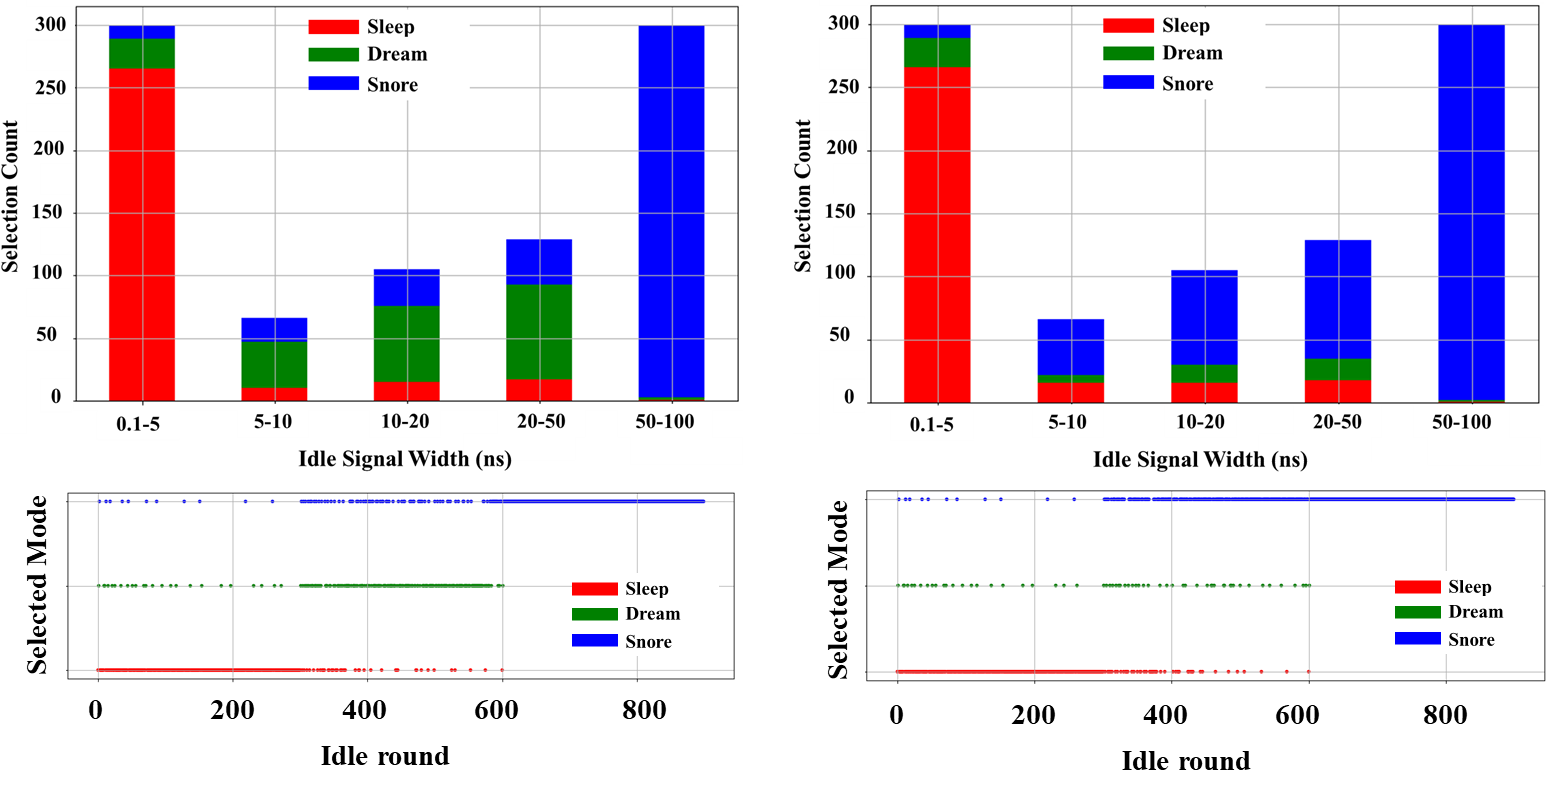
\includegraphics[width=\linewidth]{PVT.png}
    \caption{Mode selection trends corresponding to various idle time intervals.}
    \label{Bins}
\end{figure*}

To validate the controller, an idle signal pattern of 900 samples is generated with idle durations ranging from 0.1 ns to 100 ns. When subjected to this periodic and dynamically variable idle input, the bandit-based controller initially explores all available power modes and progressively converges toward the mode offering the highest reward, thus balancing leakage savings and wake-up latency. In this scenario, the controller exhibits a bias toward minimizing wake-up latency. Particularly, the controller selects the Sleep mode for brief idle intervals, transitions to the Dream mode for medium durations, and opts for the Snore mode during extended idle periods, ss shown in Fig.~\ref{Bins}. Some degree of exploration persists within each bin before the controller consistently exploits the optimal mode.

With this adaptive selection mechanism, the total leakage energy across the input test pattern is 0.493 pJ. In contrast, maintaining a single state-retentive mode (e.g., Sleep mode only in \cite{patent}), results in 1.45 pJ of leakage energy for the same input pattern. This result demonstrates an additional 66\%  reduction in leakage energy while preserving responsiveness through dynamic mode selection.

\section{Conclusion}
This work presents a low-overhead, multi-mode power gating architecture with a machine learning-based controller that adaptively reduces leakage power in idle-prone systems. Designed in 65 nm CMOS technology node with full state retention, the proposed approach achieves up to 98\% leakage savings and 71.7\% improvement over SOTA approaches. The solution is robust to process variations and suitable for 2.5D/3D HPC systems.

\vspace{-5pt}


\bibliography{References}
\bibliographystyle{ieeetr}


\end{document}
